\section{Experiment 10H: higher-order LPV sharing gate}
\label{sec:experiment10h}

\paragraph{Redesign objective.}
Experiment 10G showed that broader vehicle classes alone do not strengthen the
FL argument: a pooled LQI controller remained robust, while exact nominal
specialization could be less robust near nonlinear constraints. Experiment
10H therefore changes the information problem without changing the control
paradigm. It retains speed-scheduled LQI but introduces dynamic tire-force and
steering-actuator states that require richer speed--frequency excitation. The
claim under test is that fleet sharing can compensate for realistically
incomplete local calibration coverage.

\paragraph{Higher-order LPV plant.}
The state is
\begin{equation}
 x=[\beta,r,f_{yf},f_{yr},\delta_a]^\top,
 \qquad f_{yf}=F_{yf}/m,\quad f_{yr}=F_{yr}/m.
\end{equation}
Normalizing tire forces by mass keeps the state numerically well scaled. The
lateral motion is
\begin{equation}
 \dot\beta=\frac{f_{yf}+f_{yr}}{v_x}-r,
 \qquad
 \dot r=\frac{m(l_f f_{yf}-l_r f_{yr})}{I_z}.
\end{equation}
Front and rear force dynamics use relaxation lengths $\sigma_f,\sigma_r$,
\begin{align}
 \dot f_{yf}&=\frac{v_x}{\sigma_f}
 \left[\frac{C_f}{m}\left(\delta_a-\beta-\frac{l_fr}{v_x}\right)-f_{yf}\right],\\
 \dot f_{yr}&=\frac{v_x}{\sigma_r}
 \left[\frac{C_r}{m}\left(-\beta+\frac{l_rr}{v_x}\right)-f_{yr}\right],
\end{align}
and $\dot\delta_a=(\delta_{\rm cmd}-\delta_a)/\tau_\delta$. Compact, SUV,
and sport centers retain the 10G mass, inertia, geometry, stiffness, and
actuator values. Their front/rear relaxation-length centers are
$(0.42,0.50)$, $(0.82,0.95)$, and $(0.25,0.30)$~m, respectively, with bounded
within-class scatter.

The primary simulation plant is the exact time-varying LPV system, evaluated
by interpolating its exact discrete matrices over 10--30~m/s. This intentionally
removes tire saturation as a confounder. Nonlinear robustness is deferred
until the sharing mechanism has passed an oracle gate.

\paragraph{Complementary information audit.}
Each client observes one of four contiguous speed blocks and one of three
steering-frequency bands. The matrix-valued LPV regression uses five speed
basis functions and the six-dimensional regressor $[x^\top,u]^\top$, hence it
requires rank 30. Even with noise-free full-state data, local designs have rank
12--18 and are structurally deficient. Pooling ten clients within a class
produces rank 30 in every fleet. After column normalization, aggregate design
conditions have median $1.28\times10^5$ and maximum $2.58\times10^5$. Thus
sharing adds missing directions rather than merely averaging repeated data.

\paragraph{Controller and protocol.}
The LQI state augments the five plant states with integrated yaw-rate error.
Four weight candidates are selected on development seeds 461--465 using only
ClientExact models. The frozen choice is
\begin{equation}
 Q=\operatorname{diag}(50,75,0.05,0.05,5,1500),\qquad R=0.2.
\end{equation}
All candidates are stable and feasible. Evaluation uses a speed-varying
broadband reference containing 0.35, 0.9, and 1.35~Hz components and a
three-pulse transient.

An initial oracle-class pilot on seeds 471--480 found that Global was already
better than OracleClass. Those seeds are excluded from the final sharing
comparison and retained in the repository. The revised endpoint compares
Global with LocalRestricted, which uses each client's exact noise-free matrices
at its observed speeds and nearest-speed extrapolation elsewhere. This is an
optimistic local baseline. The revised protocol was frozen before running
untouched seeds 481--490.

\begin{table}[htbp]
\centering
\caption{Experiment 10H confirmation yaw-rate RMSE in deg/s, averaged over ten fresh fleets.}
\label{tab:experiment10h-summary}
\begin{tabular}{llrr}
\toprule
Maneuver & Method & Mean client & Worst client\\
\midrule
Broadband & LocalRestricted & 0.16820 & 0.25026\\
Broadband & Global          & 0.15235 & 0.21319\\
Broadband & OracleClass     & 0.15575 & 0.22165\\
Broadband & ClientExact     & 0.15504 & 0.21141\\
\midrule
Transient & LocalRestricted & 0.13484 & 0.19952\\
Transient & Global          & 0.13140 & 0.17205\\
Transient & OracleClass     & 0.13823 & 0.19779\\
Transient & ClientExact     & 0.13719 & 0.18804\\
\bottomrule
\end{tabular}
\end{table}

\begin{table}[htbp]
\centering
\caption{Global improvement over LocalRestricted. Positive values favor sharing.}
\label{tab:experiment10h-comparison}
\begin{tabular}{llrrr}
\toprule
Maneuver & Endpoint & Improvement & 95\% CI & Fleet wins\\
\midrule
Broadband & Mean client  & 9.42\%  & [9.13,9.71]\%   & 10/10\\
Broadband & Worst client & 14.71\% & [12.17,17.21]\% & 10/10\\
Transient & Mean client  & 2.55\%  & [2.43,2.67]\%   & 10/10\\
Transient & Worst client & 13.65\% & [11.09,16.23]\% & 10/10\\
\bottomrule
\end{tabular}
\end{table}

\begin{figure}[htbp]
\centering
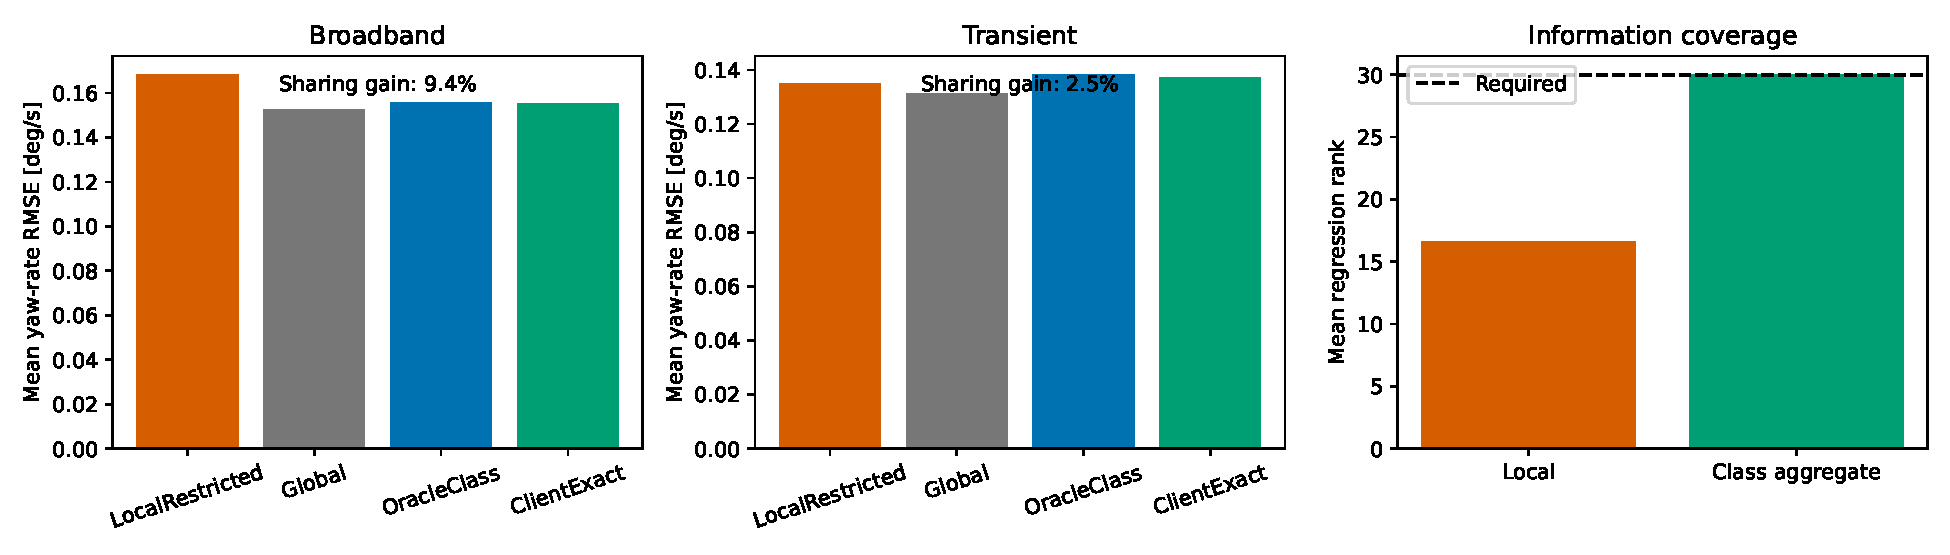
\includegraphics[width=0.98\linewidth]{../results/figures/experiment_10h_higher_order_lpv_gate.pdf}
\caption{Experiment 10H matched-LPV control and information-coverage audit.}
\label{fig:experiment10h}
\end{figure}

\paragraph{Result and interpretation.}
Complementary sharing produces a genuine closed-loop benefit. Global beats the
optimistic LocalRestricted baseline in every fleet and endpoint, with positive
paired intervals. The effect is strongest in the fleet tail: worst-client
tracking improves by 14.71\% and 13.65\%. Mean broadband tracking improves by
9.42\%. Mean transient tracking improves by only 2.55\%, so the deliberately
strict requirement of at least 5\% on every endpoint fails. Experiment 10H
therefore supports a strong calibration-coverage and worst-client claim, not a
uniformly large nominal-mean claim.

Global is also within the predefined 5\% envelope of ClientExact on every
endpoint and sometimes has lower yaw-only RMSE because pooling regularizes the
fixed LQI design. OracleClass is worse than Global, confirming that physical
class specialization is not needed for this control objective. The emerging
FL story is consequently shared full-envelope LPV backbone identification,
not clustered controller deployment.

\paragraph{Decision.}
The higher-order model resolves the core information-sharing problem without
leaving LPV/LQI control. The next experiment should estimate this model from
finite noisy local trajectories and compare LocalRestricted, centralized
pooled, federated pooled, LocalFull, and ClientExact under a calibration-time
budget. The primary endpoint should be worst-client tracking and the amount of
local excitation needed to reach a target performance. Learned clustering
should be reintroduced only if finite-data diagnostics show that Global pooling
becomes biased.

\paragraph{Reproducibility.}
Configuration, implementation, and tests are in
\path{code/config/experiment_10h.json}. The implementation is in
\path{code/experiments/experiment_10h_higher_order_lpv_gate.py}; tests are in
\path{code/tests/test_experiment_10h.py}. Development selection, the disclosed
pilot, final client-level records, coverage diagnostics, paired comparisons,
gate decisions, and provenance hashes are stored under \path{results}.
